\documentclass[12pt]{article}

\usepackage{fullpage}
\usepackage{mdframed}
\usepackage{colonequals}
\usepackage{algpseudocode}
\usepackage{algorithm}
\usepackage{tcolorbox}
\usepackage[all]{xy}
\usepackage{proof}
\usepackage{mathtools}
\usepackage{bbm}
\usepackage{amssymb}
\usepackage{amsthm}
\usepackage{amsmath}
\usepackage{amsxtra}
\newcommand{\bb}{\mathbb}


\newtheorem{theorem}{Theorem}[section]
\newtheorem{corollary}{Corollary}[theorem]
\newtheorem{lemma}{Lemma}

\newcommand{\mathcat}[1]{\textup{\textbf{\textsf{#1}}}} % for defined terms

\newenvironment{problem}[1]
{\begin{tcolorbox}\noindent\textbf{Problem #1}.}
{\vskip 6pt \end{tcolorbox}}

\newenvironment{enumalph}
{\begin{enumerate}\renewcommand{\labelenumi}{\textnormal{(\alph{enumi})}}}
{\end{enumerate}}

\newenvironment{enumroman}
{\begin{enumerate}\renewcommand{\labelenumi}{\textnormal{(\roman{enumi})}}}
{\end{enumerate}}

\newcommand{\defi}[1]{\textsf{#1}} % for defined terms

\theoremstyle{remark}
\newtheorem*{solution}{Solution}

\setlength{\hfuzz}{4pt}

\newcommand{\calC}{\mathcal{C}}
\newcommand{\calF}{\mathcal{F}}
\newcommand{\C}{\mathbb C}
\newcommand{\N}{\mathbb N}
\newcommand{\Q}{\mathbb Q}
\newcommand{\R}{\mathbb R}
\newcommand{\Z}{\mathbb Z}
\newcommand{\br}{\mathbf{r}}
\newcommand{\RP}{\mathbb{RP}}
\newcommand{\CP}{\mathbb{CP}}
\newcommand{\nbit}[1]{\{0, 1\}^{#1}}
\newcommand{\bits}{\{0, 1\}^{n}}
\newcommand{\bbni}{\bigbreak \noindent}
\newcommand{\norm}[1]{\left\vert\left\vert#1\right\vert\right\vert}

\let\1\relax
\newcommand{\1}{\mathbf{1}}
\newcommand{\fr}[2]{\left(\frac{#1}{#2}\right)}

\newcommand{\vecz}{\mathbf{z}}
\newcommand{\vecr}{\mathbf{r}}
\DeclareMathOperator{\Cinf}{C^{\infty}}
\DeclareMathOperator{\Id}{Id}

\DeclareMathOperator{\Alt}{Alt}
\DeclareMathOperator{\ann}{ann}
\DeclareMathOperator{\codim}{codim}
\DeclareMathOperator{\End}{End}
\DeclareMathOperator{\Hom}{Hom}
\DeclareMathOperator{\id}{id}
\DeclareMathOperator{\M}{M}
\DeclareMathOperator{\Mat}{Mat}
\DeclareMathOperator{\Ob}{Ob}
\DeclareMathOperator{\opchar}{char}
\DeclareMathOperator{\opspan}{span}
\DeclareMathOperator{\rk}{rk}
\DeclareMathOperator{\sgn}{sgn}
\DeclareMathOperator{\Sym}{Sym}
\DeclareMathOperator{\tr}{tr}
\DeclareMathOperator{\img}{img}
\DeclareMathOperator{\CandE}{CandE}
\DeclareMathOperator{\CandO}{CandO}
\DeclareMathOperator{\argmax}{argmax}
\DeclareMathOperator{\first}{first}
\DeclareMathOperator{\last}{last}
\DeclareMathOperator{\cost}{cost}
\DeclareMathOperator{\dist}{dist}
\DeclareMathOperator{\path}{path}
\DeclareMathOperator{\parent}{parent}
\DeclareMathOperator{\argmin}{argmin}
\DeclareMathOperator{\excess}{excess}
\let\Pr\relax
\DeclareMathOperator{\Pr}{\mathbf{Pr}}
\DeclareMathOperator{\Exp}{\mathbb{E}}
\DeclareMathOperator{\Var}{\mathbf{Var}}
\let\limsup\relax
\DeclareMathOperator{\limsup}{limsup}
%Paired Delims
\DeclarePairedDelimiter\ceil{\lceil}{\rceil}
\DeclarePairedDelimiter\floor{\lfloor}{ \rfloor}


\newcommand{\dagstar}{*}

\newcommand{\tbigwedge}{{\textstyle{\bigwedge}}}
\setlength{\parindent}{0pt}
\setlength{\parskip}{5pt}


\begin{document}

\title{CS 40: Computational Complexity}

\author{Sair Shaikh}
\maketitle

% Collaboration Notice: Talked to Henry Scheible '26 to discuss ideas.



\begin{problem}{1}
    Consider the chain complexes $C$ and $D$ given by 
\[ C_i = \begin{cases} \Z/2\Z & i = 0 \\ 0 & i \neq 0 \end{cases} \hspace{2 cm}  D_i = \begin{cases} \Z & i = 0,1 \\ 0 & i \neq 0,1 \end{cases} \]
where all the differentials on $C$ is zero and $\partial_1(n)= 2n$ on $D$. Show that $C$ and $D$ are quasi-isomorphic (have isomorphic homology) but are not chain homotopy equivalent.
\end{problem}
\begin{solution}
    We write down the chain complexes explicitly: 
    \begin{align*}
        C: 0 \to &\Z/2\Z \xrightarrow{0} 0 \to 0 \\
        D: 0 \to &\Z \xrightarrow{2} \Z \xrightarrow{0} 0
    \end{align*}
    Then, we compute the homology of $C$ and $D$:
    \begin{align*}
        H_0(C) &= \ker(\Z/2\Z \to 0)/\img(0 \to \Z/2\Z) = \Z/2\Z \\
        H_k(C) &= 0 \text{ for } k \neq 0 \\
        H_1(D) &= \ker(\Z \xrightarrow{2} \Z)/\img(0 \to \Z) = 0 \\
        H_0(D) &= \ker(\Z \to 0)/\img(\Z \xrightarrow{2} \Z) = \Z/2\Z \\
        H_k(D) &= 0 \text{ for } k \neq 0,1
    \end{align*}
    Thus, the homology groups of $C$ and $D$ are isomorphic. Thus, $C$ and $D$ are quasi-isomorphic. However, note that if we had a chain homotopy equivalence, we would have maps $f: C \to D$ and $g: D \to C$ such that $f \circ g$ is chain homotopic to $\id_D$. However, this would imply that $f_0 \circ g_0$ is chain homotopic to $\id_{D_0} = \id_{\Z}$. However, $f_0: \Z/2\Z \to \Z$ must be the zero map. Thus, $f_0 \circ g_0$ is also zero, which is not chain homotopic to $\id_\Z$.
\end{solution}
\newpage

\begin{problem}{2}
     If $p \colon E \to B$ is a covering map, we know it induces an injective map on fundamental groups. Is the same true for the map $H_1(E) \to H_1(B)$?
\end{problem}
\begin{solution}
    Let $B = S^1 \vee S^1$ and $E$ be the following covering space from class. \bbni
    \begin{centering}
    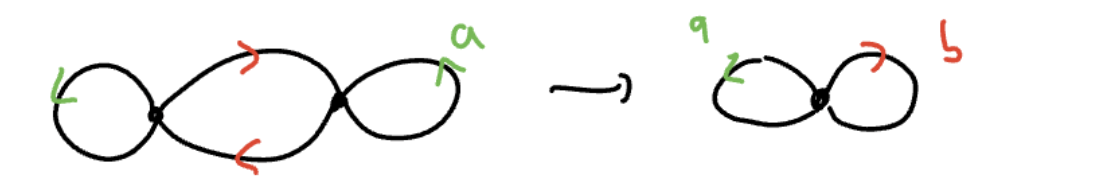
\includegraphics[width=0.8\textwidth]{assets/hwk7_cover.png}
    \end{centering} \bbni
    Then, note that $\pi_1(E) = F_3$ and $\pi_1(B) = F_2$, where $F_n$ is the free group on $n$ generators. Moreover, as $E$ and $B$ are path-connected, $H_1$ is the abelianization of the fundamental group. Thus, we have $H_1(E) = \Z^3$ and $H_1(B) = \Z^2$. Thus, the induced map is: 
    \[  p: \Z^3 \to \Z^2\]
    This map cannot be injective, as $\Z^3$ has a larger rank than $\Z^2$. 
\end{solution}
\newpage


\begin{problem}{3}(2.1.16) 
\begin{enumerate}
    \item Show that $H_0(X,A) = 0$ if and only if $A$ meets every path component of $X$.
    \item Show that $H_1(X,A) = 0$ if and only if $H_1(A) \to H_1(X)$ is surjective and every path component of $X$ contains at most one path component of $A$.
\end{enumerate}     
\end{problem}
\begin{solution}
    \bbni 
    \begin{enumerate}
        \item Note that we have the long exact sequence, ending in:
        \[ H_1(X, A) \to H_0(A) \xrightarrow{\iota_*} H_0(X) \to H_0(X, A) \to 0 \]
        Moreover, if $X_i$ for $i \in I$ are the path components of $X$, then we also have: 
        \[ H_0(X) = \bigoplus_{i \in I} H_0(X_i) \]
        Where $H_0(X_i) \cong \Z$ as they are path-connected. Finally, note that if $[\sigma] = [\sigma']$ in $H_0(\cdot)$, $\sigma' - \sigma$ is a boundary if and only if the images of $\sigma$ and $\sigma'$ (single points) have a path connecting them, i.e. are in the same path component. \bbni
        Assume $H_0(X, A) = 0$. Then, we have that $\iota_*: H_0(A) \to H_0(X)$ is surjective. Thus, if $\sigma_i: \Delta_0 \to X_i$ is a representative of the generator of $H_0(X_i)$, we have a $\tau_i: \Delta_0 \to A$ such that $\iota_*([\tau_i]) = [\sigma_i]$. Thus, we have that $[\iota \circ \tau_i] = [\sigma_i]$. Thus, the point picked out by $\iota \circ \tau_i$ is in the same path-component as the image of $\sigma_i$, i.e. $X_i$. However, as $\iota$ is the inclusion map, this means the image of $\tau_i$ is in $A \cap X_i$. Thus, $A$ meets every path component of $X$. \bbni
        Conversely, assume that $A$ meets every path component of $X$. We show that $\iota_*$ is surjective. Let $[\sigma_i]$ be a generator of $H_0(X_i)$. Since $A$ meets every path component of $X$, there exists a point $x_i \in A \cap X_i$. Then, we can take $\tau_i: \Delta_0 \to A$ to be the map picking out $x_i$. Then, we have that: 
        \[ \iota_*([\tau_i]) = [\iota \circ \tau_i] = [\sigma_i]\]
        as the image of $\iota \circ \tau_i$ and $\sigma_i$ are in the same path component $X_i$. Thus, $\iota_*$ maps to each generator of $H_0(X)$ and is thus surjective. Thus, the long exact sequence above implies that $H_0(X, A) = 0$. 
        \item Consider the end of same long exact sequence as above: 
        \[ \cdots \to H_1(A) \xrightarrow{\iota_*} H_1(X) \to H_1(X, A) \to H_0(A) \xrightarrow{\iota_*} H_0(X) \to H_0(X, A) \to 0 \]
        Assume $H_1(X, A) = 0$. Then, the sequence breaks into two exact sequences:
        \begin{align*}
            &\cdots \to H_1(A) \xrightarrow{\iota_*} H_1(X) \to 0 \\
            &0 \to H_0(A) \xrightarrow{\iota_*} H_0(X) \to H_0(X, A) \to 0
        \end{align*}
        Then, we have that $\iota_*: H_1(A) \to H_1(X)$ is surjective and that $\iota_*: H_0(A) \to H_0(X)$ is injective. Now let $X_i$ be a path-component of $X$. Assume $X_i$ contains at least one path-component of $A$. Then let $A_i$ and $A_j$ be path-components of $A$ contained in $X_i$. Then, let $\tau_i: \Delta_0 \to A_i$ and $\tau_j: \Delta_0 \to A_j$ be two maps picking out a point in $A_i$ and $A_j$ respectively. Then, note that $\iota_*([\tau_i]) = [\iota \circ \tau_i]$ and $\iota_*([\tau_j]) = [\iota \circ \tau_j]$ both pick out a point in $X_i$. Since $X_i$ is path-connected, this implies:
        \[\iota_*([\tau_i]) = \iota_*([\tau_j])\]
        As $\iota_*$ is injective, this implies that $[\tau_i] = [\tau_j]$. Thus, $A_i$ and $A_j$ are in the same path-component, i.e. are equal. \bbni 
        On the other hand, assume that $\iota_*: H_1(A) \to H_1(X)$ is surjective and that every path component of $X$ contains at most one path component of $A$. Then, we first show that $\iota_*: H_0(A) \to H_0(X)$ is injective. \bbni
        Let $\tau_i: \Delta_0 \to A$ and $\tau_j: \Delta_0 \to A$ be two maps picking out points in $A$ such that: 
        \[ \iota_*([\tau_i]) = \tau_*([\tau_j])\]
        Then, we have that $[\iota \circ \tau_i] = [\iota \circ \tau_j]$. Thus, the points picked out by $\iota \circ \tau_i$ and $\iota \circ \tau_j$ are in the same path component of $X$, call it $X_i$. However, as $\tau_i$ and $\tau_j$ pick out points in path-components of $A$ contained in $X_i$. By assumption, there is at most one such path-component (in this case exactly one, as we know there exists one). Thus, $\tau_i$ and $\tau_j$ pick points in the same path-component of $A$. Thus, $[\tau_i] = [\tau_j]$ and $\iota_*$ is injective. \bbni
        Consider the long exact sequence again. We have that:
        \[ \cdots \to H_1(A) \xrightarrow{\iota_*} H_1(X) \to H_1(X, A) \to H_0(A) \xrightarrow{\iota_*} H_0(X) \to H_0(X, A) \to 0 \]
        Then, as $\iota_*: H_1(A) \to H_1(X)$ is surjective, we have that:
        \[\ker(H_1(X) \to H_1(X,A)) = \img(H_1(A) \to H_1(X)) = H_1(X)\]
        Thus, the map $H_1(X) \to H_1(X, A)$ is the zero map. Thus, we have:
        \[ \cdots \to H_1(A) \xrightarrow{\iota_*} H_1(X) \xrightarrow{0} H_1(X, A) \to H_0(A) \xrightarrow{\iota_*} H_0(X) \to H_0(X, A) \to 0 \]   
        Continuing on, this implies:
        \[ \ker(H_1(X, A) \to H_0(A)) = \img(H_1(X) \to H_1(X, A)) = 0\]
        Thus, the map $H_1(X, A) \to H_0(A)$ is injective. However, finally, as $\iota_*: H_0(A) \to H_0(X)$ is injective, we have that:
        \[\img(H_1(X, A) \to H_0(A)) = \ker(H_0(A) \to H_0(X)) = 0\]
        Thus, the map $H_1(X, A) \to H_0(A)$ is an injective map with $0$ as its image, and we must have that $H_1(X, A) = 0$.
    \end{enumerate}
\end{solution}
\newpage


\begin{problem}{4}
    Use the Mayer-Vietoris sequence to compute
    \begin{enumerate}
        \item all homology groups of a bouquet of circles $\vee^n S^1$.  
        \item all homology groups of the oriented surface of genus $g$, $M_g$. 
        \item all homology groups of the non-oriented surface of genus $k$, $N_k$
        \item $H_1(S^3 \setminus K)$ where $K$ is a knot in $S^3$. (\emph{Note:} A knot is the homeomorphic image of a circle. You can use the fact that every knot has a `tubular neighborhood' homeomorphic to the interior of a solid torus.)
    \end{enumerate}
\end{problem}
\begin{solution}
    \bbni
    \begin{enumerate}
        \item We do this via induction. Let $X = \bigvee^n S^1$. We claim that the homology groups for $X$ are: 
        \[ H_k(X) \cong \begin{cases} \Z & k = 0 \\ \Z^n & k = 1 \\ 0 & k \geq 2 \end{cases} \]
        For $n = 1$, we have that $X = S^1$, and we know the homology groups are:
        \[ H_k(X) = \begin{cases} \Z & k = 0, 1 \\ 0 & k \geq 2 \end{cases} \]
        Next, let $n > 1$. Let $X= \bigvee^n S^1$. Let $A = \bigvee^{n-1} S^1$ and $B = S^1$ (the final circle), . Then, we have that $X = \text{int}(A) \cup \text{int}(B)$ and $A \cap B = \{*\}$ is a single point. We have the Mayer-Vietoris sequence:
        \[ \cdots \to H_k(A) \oplus H_k(B) \to H_k(X) \to H_{k-1}(A \cap B) \to H_{k-1}(A) \oplus H_{k-1}(B) \to \cdots\]
        For $k \geq 2$, we have that $H_k(A) = H_k(B) = 0$. Moreover, as $k-1 \geq 1$, we have that $H_{k-1}(A \cap B) = 0$. Thus, we reduce to:
        \[ 0 \to H_k(X) \to 0 \]
        Thus, $H_k(X) = 0$ for $k \geq 2$. \bbni
        For $k = 1$, we use the induction hypothesis to note $H_1(A) = \Z^{n-1}$ and $H_0(A) = \Z$. Moreover, $H_1(B) = H_0(B) = \Z$, $H_0(A \cap B) = \Z$, and $H_1(A \cap B) = 0$. Thus, we have: 
        \[ \cdots \to 0 \to \Z^{n-1} \oplus \Z \to H_1(X) \to \Z \to \Z \oplus \Z \cdots\]
        The final map is the diagonal inclusion map between $H_0$, i.e. it maps $1 \to (1, 1)$. Thus, the kernel of this map is trivial. Thus, the image of the previous map is trivial, i.e. the map $H_1(X) \to \Z$ is zero. Thus, the map $\Z^{n-1} \oplus \Z \to H_1(X)$ is surjective. Moreover, the kernel of this map is trivial as the image of the previous map is trivial. Thus, we have that $H_1(X) \cong \Z^n$. \bbni
        For $k = 0$, we have that $H_0(A) = H_0(B) = H_0(A\cap B) = \Z$, thus we have the sequence:  
        \[ \cdots \to \Z \to \Z \oplus \Z \to H_0(X) \to 0\]
        The first map is the diagonal inclusion map $1 \to (1, 1)$. Thus, the image of this map is isomorphic to $\Z$. Thus, the kernel of the map $\Z \oplus \Z \to H_0(X)$ is isomorphic to $\Z$. Moreover, this map is surjective, as the image of the next map is trivial. By rank-nullity, we have that $H_0(X) \cong \Z$. \bbni
        This finishes the induction. 
        \item Let $M_g$ be the oriented surface of genus $g$. We claim that the homology groups are: 
        \[ H_k(M_g) = \begin{cases} \Z & k = 0 \\ \Z^{2g} & k = 1 \\ \Z & k = 2 \\ 0 & k \geq 3 \end{cases} \]
        Let $U$ be all but a small disk on the left-most side of the surface. Let $V$ be a slightly larger than the complement of $U$. Then, clearly $\text{int}(U) \cup \text{int}(V) = M_g$. Moreover, we have that $U \cap V$ is homotopic to $S^1$ and $U$ is homotopic to $\bigvee^{2g} S^1$ (CW complex picture), and $V$ is contractible to a point. Next, consider the Mayer-Vietoris sequence:
        \[ \cdots \to H_k(U \cap V) \to H_k(U) \oplus H_k(V) \to H_k(X) \to H_{k-1}(U \cap V)  \to \cdots\]
        For $k = 0$, we have that $H_0(U) = H_0(V) = H_0(U \cap V) = \Z$. Thus, the sequence reduces to: 
        \[ \cdots \to \Z \to \Z \oplus \Z \to H_0(X) \to 0 \]
        Then the map $\Z \to \Z \oplus \Z$ is the diagonal inclusion map $1 \to (1, 1)$ (similar to the first part). Thus, the image of this map is isomorphic to $\Z$, thus the kernel of the next map is isomorphic to $\Z$. By rank-nullity, the image of the next map is isomorphic to $\Z$. However, the map $\Z \oplus \Z \to H_0(X)$ is surjective, thus $H_0(X) \cong \Z$. \bbni
        For $k = 1$, we have that $H_1(U) = \Z^{2g}$, $H_1(V) = 0$ (abelinization of $0$), $H_0(U \cap V) = H_1(U \cap V) = \Z$, and $H_0(U) \oplus H_0(V) = \Z^2$. Thus, we have the sequence:
        \[ \cdots \to \Z \to \Z^{2g} \oplus 0 \to H_1(X) \to \Z  \to \Z^2  \to \cdots\]    
        Similar to before, the map $\Z \to \Z^2$ is injective, thus has trivial kernel. Thus the previous map is $0$. Thus, the map $\Z^{2g} \to H_1(X)$ is surjective. \bbni
        We consider carefully the map $H_1(U \cap V) \to H_1(U) \oplus H_1(V)$, i.e. $\Z \to \Z^{2g}$. In the CW picture, $X$ is obtained from attaching a $2$-cell, along $U \cap V$ to $U$. The generator of $H_1(U \cap V)$ then maps to the boundary of $U$ in the CW-complex picture, which contains a path around each circle twice, with opposite signs. Thus, the image of this map is $0$. Thus, the map $\Z^{2g} \to H_1(X)$ is also injective. Thus, we have that:
        \[ H_1(X) \cong \Z^{2g}\]
        For $k = 2$, we have that $H_2(U) = 0$ (part a), $H_2(V) = 0$ (contractible), $H_1(U \cap V) = \Z$. Thus, we have the sequence:
        \[ \cdots \to 0 \to H_2(X) \to \Z \to \Z^2 \]
        As we previously argued, the final map $\Z \to \Z^2$ is the zero map, thus the map $H_2(X) \to \Z$ is surjective. It is also injective as the image of the previous map is trivial. Thus, we have that $H_2(X) \cong \Z$. \bbni
        For $k \geq 3$, we have that $H_k(U) = H_k(V) = 0$. Moreover, as $k-1 \geq 2$, we have that $H_{k-1}(U \cap V) = 0$. Thus, the sequence reduces to:
        \[ \cdots \to 0 \to H_k(X) \to 0 \to \cdots\]
        Thus, $H_k(X) = 0$ for $k \geq 3$.
        \[ H_k(M_g) \cong \begin{cases} \Z & k = 0 \\ \Z^{2g} & k = 1 \\ \Z & k = 2 \\ 0 & k \geq 3 \end{cases} \]

        \item Consider the CW-complex picture. Let $U$ be all but a disk in the middle of the $2$-cell. Let $V$ be a slightly larger disk than the complement of $U$. Then, we have that $\text{int}(U) \cup \text{int}(V) = N_k$. Moreover, we have that $U \cap V$ is homotopic to $S^1$ and $U$ is homotopic to $\bigvee^{k} S^1$, and $V$ is contractible to a point. Next, consider the Mayer-Vietoris sequence:
        \[ \cdots \to H_k(U \cap V) \to H_k(U) \oplus H_k(V) \to H_k(X) \to H_{k-1}(U \cap B) \to \cdots\]
        For $k = 0$, we have that $H_0(U) = H_0(V) = H_0(U \cap V) = \Z$. Moreover, the map $H_0(U \cap V) \to H_0(U) \oplus H_0(V)$ is the diagonal inclusion map $1 \to (1, 1)$. Thus, we have: 
        \[ \cdots \to \Z \to \Z^2 \to H_0(X) \to 0\]
        and the map $\Z^2 \to H_0(X)$ has image isomorphic to $\Z$ and is surjective, thus, $H_0(X) \cong \Z$. \bbni
        For $k = 1$, we have that $H_1(U) = \Z^k$, $H_1(V) = 0$, $H_1(U \cap V) = \Z$, and $H_0$ of everything is $\Z$. Thus, we have the sequence:
        \[ \cdots \to \Z \to \Z^k \oplus 0 \to H_1(X) \to \Z \to \Z^2\]
        Similar to before, consider the map $H_1(U \cap V) \to H_1(U)$ i.e. $\Z \to \Z^k$. The generator of $H_1(U \cap V)$ maps to the boundary of $U$ in the CW-complex picture, which contains a copy of each of the $k$ circles twice each with the same signs. Thus, this maps: 
        \[ 1 \to (2, \cdots, 2)\] 
        Thus, the image of this map is isomorphic to $2\Z$. Thus, the kernel of the map $\Z^k \to H_1(X)$ is isomorphic to $2\Z$. Using the first isomorphism theorem, the image of the map is isomorphic to $\Z^k/2\Z \cong \Z^{k-1}\oplus \Z/2\Z$. \\
        Moreover, as noted before, the map $H_1(U \cap V) \to H_1(U) \oplus H_1(V)$ is the diagonal inclusion map, which is injective, thus has $0$ kernel. Thus, the image of $H_1(X) \to \Z$ is $0$. Thus, the map $\Z^k \to H_1(X)$ is surjective. Thus, we have that $H_1(X) \cong \Z^{k-1} \oplus \Z/2\Z$. \bbni
        For $k = 2$, we have that $H_2(U) = 0$ (part a), $H_2(V) = 0$ (contractible), $H_1(U \cap V) = \Z$, $H_1(U)\oplus H_1(V) = \Z^k$. Thus, we have the sequence:
        \[ \cdots \to 0 \to H_2(X) \to \Z \to \Z^k \]
        By previous discussion, the map $\Z \to \Z^k$ is injective, thus has $0$ kernel. Thus, the map $H_2(X) \to \Z$ is $0$. However, this map is injective as the image of the previous map is trivial. Thus, we have that $H_2(X) = 0$. \bbni
        For $k \geq 3$, we have that $H_k(U) = H_k(V) = 0$ and $H_{k-1}(U \cap V) = 0$ (as $k-1 \geq 2$). Thus, the sequence reduces to:
        \[ \cdots \to 0 \to H_k(X) \to 0\]
        Thus, $H_k(X) = 0$ for $k \geq 3$. \bbni
        Overall, the homology groups are:
        \[ H_k(N_g) \cong \begin{cases} \Z & k = 0 \\ \Z^{g-1} \oplus \Z/2\Z & k = 1 \\ 0 & k = 2 \\ 0 & k \geq 3 \end{cases} \]

        \item Let $V$ be the tubular neighborhood of the knot $K$ (homeomorphic to a circle) and $U = H_1(S^3 \setminus K)$. Then, $\text{int}(U) \cup \text{int}(V) = S^3$ and $U \cap V$ is contractible to $T^2$. Thus, we can use the Mayer-Vietoris sequence.
        \[ \cdots \to H_k(U \cap V) \to H_k(U) \oplus H_k(V) \to H_k(S^3) \to H_{k-1}(U \cap V) \to \cdots\]
        For $k = 0$, we have that $H_0(V) = H_0(U \cap V) = H_0(S^3) = \Z$ and $H_1(S^3) = 0$. Thus, the sequence becomes:
        \[ 0 \to \Z \to H_0(U) \oplus \Z \to \Z \to 0 \]
        The map $\Z \to H_0(U) \oplus \Z$ is injective and the map $H_0(U) \oplus \Z \to \Z$ is surjective. Thus, by rank-nullity considerations, we have $H_0(U) \oplus \Z \cong \Z^2$, thus $H_0(U) \cong \Z$. \bbni
        For $k = 1$, we have that $H_2(S^3) = 0$, $H_1(U \cap V) = \Z^2$ (homeomorphic to a torus), $H_1(V) = \Z$ (a circle), and $H_1(S^3) = 0$. Thus, we have the sequence:
        \[ 0 \to \Z^2 \to H_1(U) \oplus \Z \to 0 \]
        Thus, the map $\Z^2 \to H_1(U) \otimes \Z$ is both injective and surjective. Thus, $H_1(U) \cong \Z$. \bbni
        For $k = 2$ and $3$, we write down the sequence: 
        \begin{align*}
            H_3(U\cap V) \to H_3(U) \oplus H_3(V) \to H_3(S^3) \to H_2(U \cap V) \to H_2(U) \oplus H_2(V) \to H_2(S^3)
        \end{align*}
        Note that $H_3(U \cap V) = 0$ (torus), $H_3(V) = 0$ (a circle), $H_3(S^3) = \Z$, $H_2(U \cap V) = \Z$ (torus), $H_2(V) = 0$ (a circle), and $H_2(S^3) = 0$. Thus, we have the sequence:
        \begin{align*}
            0 \to H_3(U) \oplus 0 \to \Z \to \Z \to H_2(U) \oplus 0 \to 0
        \end{align*}
        Consider carefully the map $\delta: H_3(S^3) \to H_2(U \cap V)$, i.e. $\delta: \Z \to \Z$. Let $[\alpha] \in H_3(S^3)$ be the generator. Then, we can subdivide $S^3$ such that $[\alpha] = [\beta+\gamma]$ where $\beta$ and $\gamma$ are entirely within $U$ and $V$, respectively. Then, $\delta([\alpha]) = [\partial \beta] = [\partial \gamma]$ which is in $U \cap V$. If we triangulate $S^3$, the generator is the sum of the $2$-simplices representing the triangles. We can choose a triangulation that includes a triangulation of the torus, by refining. Then, $\beta$ and $\gamma$ are then sum of the triangles in $U$ and $V$. $\partial \beta$ then is the sum of all the triangles on the torus $U \cap V$. Thus, $\delta$ maps generator to generator and $\Z \to \Z$ is the identity. \\
        Thus, the map $\Z \to H_2(U)$ is zero. Thus, $H_2(U)$ is $0$ (as this map is surjective). Similarly, $H_3(U) \to \Z$ is $0$, thus $H_3(U) \cong \Z$ (as this map is injective.) \bbni
        For $k \geq 4$, we have that $H^k(U\cap V) = 0$ (torus), $H_k(V) = 0$ (a circle), and $H_k(S^3) = 0$. Thus, we have the sequence:
        \[  0 \to H_k(U) \to 0\]
        Thus, $H_k(U) = 0$ for $k \geq 4$. \bbni
        Thus, we have:
        \[ H_k(S^3 \setminus K) \cong \begin{cases} \Z & k = 0 \\ \Z & k = 1 \\ 0 & k \geq 2 \end{cases} \]
    \end{enumerate}
\end{solution}
\newpage

\begin{problem}{5}(2.1.17)
    \begin{enumerate}
        \item Compute the homology groups $H_n(X,A)$ when $X$ is $S^2$ or $S^1 \times S^1$ and $A$ is a finite set of points in $X$.
        \item Compute the homology groups $H_n(X,A)$ and $H_n(X,B)$ for $X$ a closed orientable surface of genus $2$, $A$ is separating circle, and $B$ is a non-separating circle as depicted below. (\emph{Note:} You can use that these are good pairs and hence there is an isomorphism with homology of the quotient away from degree $0$.)
    \end{enumerate} 
    \begin{centering}
    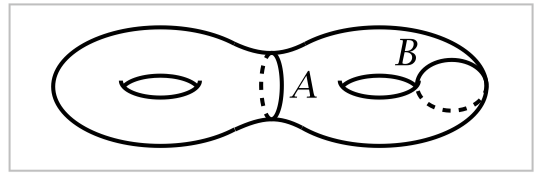
\includegraphics{assets/HW7Image.png}
    \end{centering}  
\end{problem}
\begin{solution}
    \bbni
    \begin{enumerate}
        \item Note that previous results: 
        \begin{align*}
            H_k(S^2) &= \begin{cases} \Z & k = 0, 2 \\ 0 & k \neq 0, 2\end{cases} & H_k(S^1 \times S^1) = \begin{cases} \Z & k = 0, 2 \\ \Z^2 & k = 1 \\ 
            0 & k \geq 2
        \end{cases}
        \end{align*}
        Moreover, since $A$ is a set of $n$ points, we have that: 
        \[ H_k(A) = \begin{cases} \Z^n & k = 0 \\ 0 & k \geq 1\end{cases} \]
        as it has $n$ connected components, and no non-boundary $k$-chains. 
        Note the long exact sequence: 
        \[ \cdots \to H_k(A) \xrightarrow{\iota_*} H_k(X) \to H_k(X,A) \to H_{k-1}(A) \xrightarrow{\iota_*} H_{k-1}(X) \to 0\]
        For $k = 0$, we get: 
        \[ \cdots \to H_0(A) \xrightarrow{\iota_*} H_0(X) \to H_0(X,A) \to 0\]which gives:
        \[ \cdots \to \Z^n \xrightarrow{\iota_*} \Z \to H_0(X,A) \to 0\]
        Then, note that the map $H_0(A) \xrightarrow{\iota_*} H_0(X)$ is surjective, as $H_0(X)$ is path-connected (every $0$-chain on $A$ maps to some $0$-chain on $X$, and all $0$-chains on $X$ differ by boundaries). Thus, the kernel of $\Z \to H_0(X, A)$ is trivial. Thus, this map is injective. It is followed by a $0$ map, and is thus also surjective. Thus, we have that $H_0(X, A) \cong \Z$. \bbni
        For $k = 1$, we have that:
        \[ \cdots \to H_1(A) \xrightarrow{\iota_*} H_1(X) \to H_1(X,A) \to H_0(A) \to H_0(X)\]
        which gives:
        \[ 0 \xrightarrow{\iota_*} H_1(X) \to H_1(X,A) \to \Z^n \to \Z \]      
        Since $\Z^n \to \Z$ is surjective, by rank-nullity / first isomorphism theorem, we have that the kernel of $\Z^n \to \Z$ and hence the image of $H_1(X, A) \to \Z^n$ is isomorphic to $\Z^{n-1}$. Moreover, $H_1(X) \to H_1(X, A)$ is injective, thus its image is isomorphic to $H_1(X)$. Note that for the case of $S^2$, the image is $0$ and for the case of $S^1 \times S^1$, the image is $\Z^2$. Thus, by rank-nullity, we again have:
        \[ H_1(X, A) \cong \begin{cases} \Z^{n-1} & X = S^2 \\ \Z^{n-1} \oplus \Z^2 = \Z^{n+1} & X = S^1 \times S^1\end{cases}\]
        For $k = 2$, we have that: 
        \[ \cdots \to H_2(A) \xrightarrow{\iota_*} H_2(X) \to H_2(X,A) \to H_1(A)\]
        which gives:
        \[ 0 \xrightarrow{\iota_*} \Z \to H_2(X,A) \to 0 \]
        Thus, the map $\Z \to H_2(X, A)$ is injective and surjective. Thus, $H_2(X, A) \cong \Z$. \bbni
        For $k \geq 3$, we have that both $H_k(X) = 0$ and $H_{k-1}(A) = 0$. Thus, we get that $H_k(X, A) = 0$ for $k \geq 3$. \bbni
        Overall, we summarize the results:
        \begin{align*}
            H_k(S^2, A) &= \begin{cases} \Z & k = 0 \\ \Z^{n-1} & k = 1\\ \Z& k = 2 \\ 0 & k \geq 3\end{cases} & H_k(S^1 \times S^1, A) &= \begin{cases} \Z & k = 0 \\ \Z^{n+1} & k = 1\\ \Z& k = 2 \\ 0 & k \geq 3\end{cases}
        \end{align*}       
        \item Note that since $(X, A)$ and $(X, B)$ are good pairs, we have that for $k > 0$: 
        \[ H_k(X, A) \cong \tilde{H}_k(X/A) \qquad H_k(X, B) \cong \tilde{H}_k(X/B)\]
        For the separating circle $A$, we have that $X/A = T^2 \vee T^2$. We can divide this into each open torus, $U$ and $V$, with $U \cap V$ a point. The union is clearly the whole space. Thus, we can use the Mayer-Vietoris sequence. 
        \[ H_k(U \cap V) \to H_k(U) \oplus H_k(V) \to H_k(X/A) \to H_{k-1}(U \cap V)\]
        Note that for $k \geq 3$, we have that $H_k(U) = H_k(V) = 0$ and $H_{k-1}(U \cap V) = 0$. Thus, we have:
        \[ 0 \to H_k(X/A) \to 0\]
        Thus, $H_k(X/A) = 0$ for $k \geq 3$. \bbni
        For $k = 2$, we have the following sequence:
        \[ H_2(U \cap V) \to H_2(U) \oplus H_2(V) \to H_2(X/A) \to H_{1}(U \cap V)  \]
        which gives:
        \[ 0 \to \Z \oplus \Z \to H_2(X/A) \to 0  \]
        Thus, $H_2(X/A) = \tilde H_2(X/A) \cong \Z^2$. \bbni
        For $k = 1$, we have the following sequence:
        \[ H_1(U \cap V) \to H_1(U) \oplus H_1(V) \to H_1(X/A) \to H_0(U \cap V) \to H_0(U) \oplus H_0(V) \]
        which gives:
        \[ 0 \to \Z^2 \oplus \Z^2 \to H_1(X/A) \to \Z \to \Z \oplus \Z  \]             
        as we've noted before, the final map $\Z \to \Z^2$ is the diagonal inclusion map $1 \to (1, 1)$ as $U$ and $V$ are both path-connected. Thus, the map is injective. Thus, the map $H_1(X/A) \to \Z$ is the $0$ map. Moreover, the map $\Z^2 \oplus \Z^2 \to H_1(X/A)$ is injective, thus the kernel of $H_1(X/A) \to \Z$ is the image of $\Z^2 \oplus \Z^2 \to H_1(X/A)$ is isomorphic to $Z^4$. Thus, $H_1(X/A) = \tilde H_1(X/A) \cong \Z^4$. \bbni
        Next, we consider the space $X/B$. This space is homotopic to $T^2 \vee S^1$. Let $U$ be the torus and $V$ be the circle. Then, similarly, $U \cap V$ is a point and the union of the interiors is the whole space. Thus, we can use the Mayer-Vietoris sequence. 
        \[ H_k(U \cap V) \to H_k(U) \oplus H_k(V) \to H_k(X/B) \to H_{k-1}(U \cap V)\]
        Note that for $k \geq 3$, we have that $H_k(U) = H_k(V) = 0$ and $H_{k-1}(U \cap V) = 0$. Thus, we have:
        \[ 0 \to H_k(X/B) \to 0\]
        Thus, $H_k(X/B) = 0$ for $k \geq 3$. \bbni
        For $k = 2$, we have the following sequence:
        \[ H_2(U \cap V) \to H_2(U) \oplus H_2(V) \to H_2(X/B) \to H_{1}(U \cap V)  \]
        which gives:
        \[ 0 \to \Z \oplus 0 \to H_2(X/B) \to 0  \]
        Thus, $H_2(X/B) = \tilde H_2(X/B) \cong \Z$. \bbni
        For $k = 1$, we have the following sequence:
        \[ H_1(U \cap V) \to H_1(U) \oplus H_1(V) \to H_1(X/B) \to H_0(U \cap V) \to H_0(U) \oplus H_0(V) \]
        which gives:
        \[ 0 \to \Z^2 \oplus \Z \to H_1(X/B) \to \Z \to \Z \oplus \Z  \]             
        as we've noted before, the final map $\Z \to \Z^2$ is the diagonal inclusion map $1 \to (1, 1)$ as $U$ and $V$ are both path-connected. Thus, the map is injective. Thus, the map $H_1(X/B) \to \Z$ is the $0$ map. Moreover, the map $\Z^2 \oplus \Z \to H_1(X/B)$ is injective, thus the kernel of $H_1(X/B) \to \Z$ is the image of $\Z^2 \oplus \Z \to H_1(X/B)$ is isomorphic to $Z^3$. Thus, $H_1(X/B) = \tilde H_1(X/B) \cong \Z^3$. \bbni
        Finally, for $k = 0$, we note that $H_0(X, A) = H_0(X, B) = 0$ as $X$, $A$ and $B$ are all path-connected (Problem 3). \bbni  
        Overall, we summarize the results:
        \begin{align*}
            H_k(X, A) &= \begin{cases} \Z^4 & k = 1\\ \Z^2& k = 2 \\ 0 & k \geq 3, k = 0\end{cases} & H_k(X, B) &= \begin{cases} \Z^3 & k = 1\\ \Z& k = 2 \\ 0 & k \geq 3, k =0 \end{cases}
        \end{align*}
    \end{enumerate}
\end{solution}

\end{document}